\documentclass[10pt]{beamer}

\usepackage{Theme/BeamerTheme}
\usefonttheme[onlymath]{serif}
\usepackage{hyperref}
\hypersetup{pdfpagemode=FullScreen}
\usepackage{mathrsfs}
\usepackage{amsmath}
\usepackage{bm}
\usepackage{mathtools}
\usepackage{booktabs}
\usepackage{multirow}
\usepackage{ragged2e}
\justifying
\let\raggedright\justifying
\usepackage{tikz}
\usepackage{tkz-euclide}
\usetikzlibrary{decorations.text}
\usetikzlibrary{shadows}
\usetikzlibrary{shapes}
\usetikzlibrary{circuits.logic.CDH}
\usetikzlibrary{arrows.meta}
\usetikzlibrary{decorations.pathmorphing}
\usepackage{pgfplots}
\usepgfplotslibrary{groupplots}
\usepgfplotslibrary{fillbetween}

\tikzset{
    text shadow/.code args={[#1]#2at#3(#4)#5}{
        \pgfkeysalso{/tikz/.cd,#1}%
        \foreach \angle in {0,5,...,359}{
                \node[#1,text=white] at ([shift={(\angle:.8pt)}] #4){#5};
        }
    }
}

\usepackage{tabu}
\usepackage{graphicx}
\usepackage{colortbl}

\usepackage{siunitx}
\ExplSyntaxOn
\cs_new_eq:NN \siunitx_table_collect_begin:Nn \__siunitx_table_collect_begin:Nn
\ExplSyntaxOff

\usepackage{soul}
\usepackage{keycommand}

\DeclareMathSizes{5}{5}{3}{3}

\newcommand{\pgfdefaultlinewidth}{0.75pt}
\newcommand{\risk}{\mathscr{R}}

\newkeycommand{\shadowtag}[align = center, background = white, x = 0, y = 0, color = black][1]{%
	\node at (\commandkey{x}, \commandkey{y}) [text shadow={[align=\commandkey{align}] at (\commandkey{x}, \commandkey{y}) {#1}}, align = \commandkey{align}] {\textcolor{\commandkey{color}}{#1}};
}


\begin{document}

% Cover
% \maketitle
\begin{frame}[plain, noframenumbering]\label{Title}
    \vfill
    \centering
    \usebeamerfont{title}\Huge
    Monthly Report\\
    \begin{tikzpicture}\draw[mLightBrown, line width = 1pt] (0, 0) -- (\textwidth, 0);\end{tikzpicture}\vspace{15pt}\\
    \begin{minipage}[m]{3cm}
        \Bold \small Zhang Qi
    \end{minipage}\hspace{-15pt}
    \begin{minipage}[m]{1.5cm}
        \centering
        
\includegraphics[height=0.8cm]{Logos/HUSTLogoWithoutSubline.pdf}
    \end{minipage}
    \begin{minipage}[m]{0.55\textwidth}
        \Normal \scriptsize School of Automation,\\Huazhong University of Science and Technology,\\Wuhan, China.
    \end{minipage}
    \vfill
    \centering
    \usebeamerfont{date}\usebeamercolor[fg]{date}\today
\end{frame}

% Outlines
\begin{frame}[noframenumbering]{Outlines}\label{Outlines}
    \setcounter{tocdepth}{1}
    \tableofcontents % [pausesections]
\end{frame}

% Main Body
\section{Seven Factors about the Risk}
\begin{frame}{What are the seven factors?}
    \begin{itemize}[<+->]
      \item \textbf{Attack Strategy} refers to the atom attack which is launched by an attacker to achieve his destructive purpose.
      \item \textbf{System Function} refers to the function of control system.
      \item \textbf{Security Strategy} is a kind of defense strategy which can prevent attack strategy.
      \item \textbf{Recover Strategy} is a kind of defense strategy which can recover the failed system function.
      \item \textbf{Hazardous Incident} refers to the unexpected incident which will cause monetary loss of ICSs.
      \item \textbf{Production Process} refers a manufacturing step which is a part of in a production chain.
      \item \textbf{Monetary Loss} is the sum of the loss caused by malicious attacks, the loss of production process shutdown, and the enforcement cost of defense strategy.
    \end{itemize}
\end{frame}

\begin{frame}{Seven Factors about the Risk of ICSs}
\scalebox{0.6}{
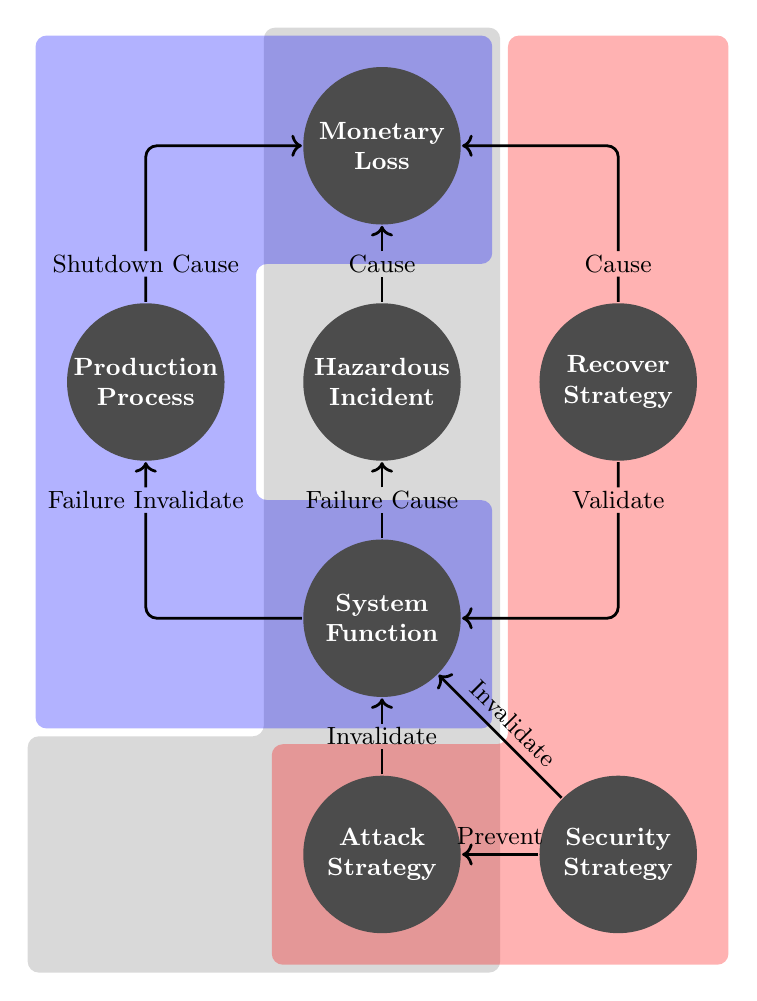
\begin{tikzpicture}[line width = 1pt,
                    factor/.style = {circle, fill = black!70, text = white, font = \bf, inner sep = 0pt, align = center, minimum size = 2cm},
                    tag/.style = {align = center, inner sep = 1pt},
                    model/.style = {rounded corners, opacity= 0.3},
                    arrow/.style = {->, rounded corners}]

\small
\fill[gray, model] (-0.5, 0.5) -- (-0.5, 3.5) -- (2.5, 3.5) -- (2.5, 12.5) -- (5.5,12.5) -- (5.5, 0.5) -- cycle;
\fill[blue, model] (-0.4, 12.4) -- (5.4, 12.4) -- (5.4, 9.5) -- (2.4, 9.5) -- (2.4, 6.5) -- (5.4, 6.5) -- (5.4, 3.6) -- (-0.4, 3.6) -- cycle;
\fill[red, model] (5.6,3.4) -- (5.6, 12.4) -- (8.4,12.4) -- (8.4, 0.6) -- (2.6, 0.6) -- (2.6, 3.4) -- cycle;


\shadowtag[x = 1, y = 2.2]{\bf Multi-level}
\shadowtag[x = 1, y = 1.8]{\bf Bayesian Network}
\shadowtag[x = 1, y = 4.2, color = blue]{\bf Process Model}
\shadowtag[x = 7, y = 4.4, color = red]{\bf Attack-Defense}
\shadowtag[x = 7, y = 4.0, color = red]{\bf Strategies Models}


\node[tag] (AS2SF) at (4, 3.5) {Invalidate};
\node[tag] (SF2HI) at (4, 6.5) {Failure Cause};
\node[tag] (SF2PP) at (1, 6.5) {Failure Invalidate};
\node[tag] (RS2SF) at (7, 6.5) {Validate};

\node[tag] (PP2ML) at (1, 9.5) {Shutdown Cause};
\node[tag] (HI2ML) at (4, 9.5) {Cause};
\node[tag] (RS2ML) at (7, 9.5) {Cause};

\node[factor] (ML) at (4, 11) {Monetary\\Loss};
\node[factor] (HI) at (4,  8) {Hazardous\\Incident};
\node[factor] (SF) at (4,  5) {System\\Function};
\node[factor] (AS) at (4,  2) {Attack\\Strategy};
\node[factor] (PP) at (1,  8) {Production\\Process};
\node[factor] (RS) at (7,  8) {Recover\\Strategy};
\node[factor] (SS) at (7,  2) {Security\\Strategy};

\draw[arrow] (AS) -- (AS2SF) -- (SF);
\draw[arrow] (SF) -- (SF2HI) -- (HI);
\draw[arrow] (HI) -- (HI2ML) -- (ML);
\draw[arrow] (SF) -| (SF2PP) -- (PP);
\draw[arrow] (PP) -- (PP2ML) |- (ML);

\draw[arrow] (RS) -- (RS2ML) |- (ML);
\draw[arrow] (RS) -- (RS2SF) |- (SF);

\draw[arrow] (SS) -- (SF) node[midway, sloped, above] {Invalidate};
\draw[arrow] (SS) -- (AS) node[midway, sloped, above] {Prevent};
\end{tikzpicture}}
\end{frame}



\section{Task Planning}
\begin{frame}{Task Planning}
    \begin{itemize}
      \item Finish the simulation of 2\textsuperscript{nd} paper.
      \item Finish the 3\textsuperscript{rd} paper for the special issue on Fuzzy Systems.
    \end{itemize}
\end{frame}




\end{document}
